\documentclass[tikz,border=10pt]{standalone}
\usepackage{lmodern}
\usepackage[T1]{fontenc}
\usepackage{tikz}
% Shared color palette for figures (not compiled on its own)
\definecolor{ink}{HTML}{1C1917}
\definecolor{crimson}{HTML}{8A1F1B}
\definecolor{navy}{HTML}{243B55}
\definecolor{gold}{HTML}{B08D3E}
\definecolor{cream}{HTML}{F7F1E8}
\definecolor{sand}{HTML}{E8DCC8}
\definecolor{mist}{HTML}{D7E1EA}
\definecolor{mid}{HTML}{6B8AA3}
\definecolor{deep}{HTML}{3D1F1E}

\begin{document}
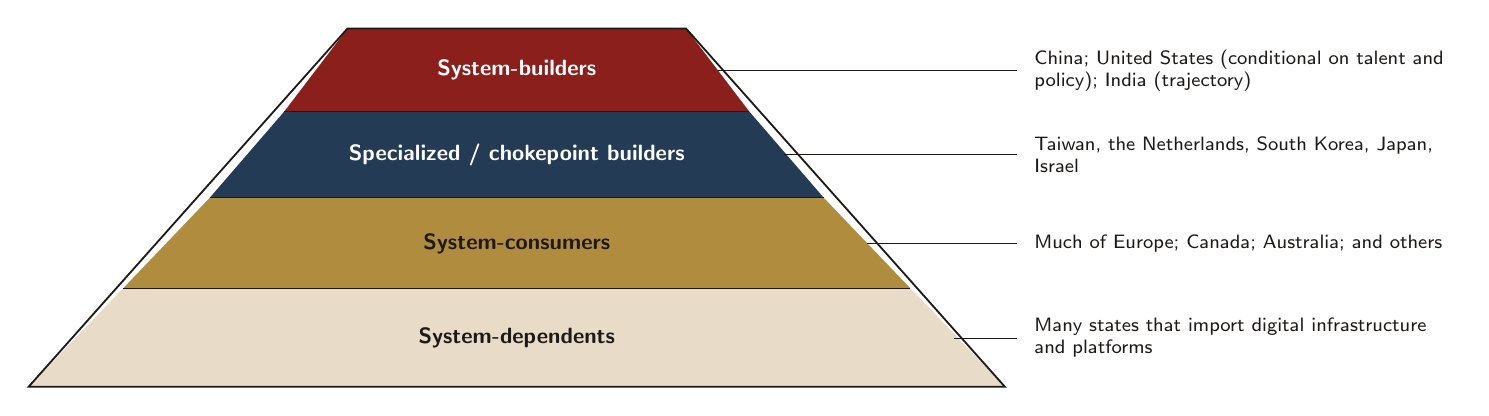
\begin{tikzpicture}[font=\sffamily, x=1cm, y=1cm]
  % Wider, slightly taller bands; short labels inside, examples to the right
  \fill[crimson] (-2.15,4.35) -- (2.15,4.35) -- (2.95,3.30) -- (-2.95,3.30) -- cycle;
  \fill[navy]    (-2.95,3.30) -- (2.95,3.30) -- (3.90,2.20) -- (-3.90,2.20) -- cycle;
  \fill[gold]    (-3.90,2.20) -- (3.90,2.20) -- (5.00,1.05) -- (-5.00,1.05) -- cycle;
  \fill[sand]    (-5.00,1.05) -- (5.00,1.05) -- (6.20,-0.20) -- (-6.20,-0.20) -- cycle;
  \draw[ink, line width=0.65pt] (-2.15,4.35) -- (2.15,4.35) -- (6.20,-0.20) -- (-6.20,-0.20) -- cycle;
  \draw[ink, line width=0.35pt] (-2.95,3.30) -- (2.95,3.30);
  \draw[ink, line width=0.35pt] (-3.90,2.20) -- (3.90,2.20);
  \draw[ink, line width=0.35pt] (-5.00,1.05) -- (5.00,1.05);
  \node[text=white, align=center, font=\sffamily\bfseries\footnotesize] at (0,3.82) {System-builders};
  \node[text=white, align=center, font=\sffamily\bfseries\footnotesize] at (0,2.75) {Specialized / chokepoint builders};
  \node[text=ink,   align=center, font=\sffamily\bfseries\footnotesize] at (0,1.62) {System-consumers};
  \node[text=ink,   align=center, font=\sffamily\bfseries\footnotesize] at (0,0.42) {System-dependents};
  % examples at right
  \node[anchor=west, text=ink, font=\sffamily\scriptsize, text width=5.3cm, align=left] at (6.45,3.82)
    {China; United States (conditional on talent and policy); India (trajectory)};
  \node[anchor=west, text=ink, font=\sffamily\scriptsize, text width=5.3cm, align=left] at (6.45,2.75)
    {Taiwan, the Netherlands, South Korea, Japan, Israel};
  \node[anchor=west, text=ink, font=\sffamily\scriptsize, text width=5.3cm, align=left] at (6.45,1.62)
    {Much of Europe; Canada; Australia; and others};
  \node[anchor=west, text=ink, font=\sffamily\scriptsize, text width=5.3cm, align=left] at (6.45,0.42)
    {Many states that import digital infrastructure and platforms};
  % leader lines
  \draw[ink, line width=0.35pt] (2.55,3.82) -- (6.35,3.82);
  \draw[ink, line width=0.35pt] (3.40,2.75) -- (6.35,2.75);
  \draw[ink, line width=0.35pt] (4.45,1.62) -- (6.35,1.62);
  \draw[ink, line width=0.35pt] (5.55,0.42) -- (6.35,0.42);
\end{tikzpicture}
\end{document}
